%==============================================================================
% Artigo 3 - FGA0261 Inteligência Artificial II - 2026.2
% Formato: IEEE conference (classe IEEEtran, máximo 4 páginas)
% Entrega: 05/11/2026, pelo Microsoft Teams
%
% CONVENÇÃO DESTE ARQUIVO: uma frase por linha.
% Compilar: make no Linux; .\build.ps1 no Windows sem Perl/latexmk.
%==============================================================================
\documentclass[conference]{IEEEtran}

\usepackage[T1]{fontenc}
\usepackage[utf8]{inputenc}
\usepackage{cite}
\usepackage{amsmath,amssymb,amsfonts}
\usepackage{graphicx}
\usepackage{booktabs}
\usepackage{url}

\graphicspath{{figs/}}

% Rótulos em português sem babel (o pacote de português não está em todas as instalações).
\renewcommand{\refname}{Referências}
\renewcommand{\tablename}{Tabela}
\renewcommand{\figurename}{Fig.}
\renewcommand{\abstractname}{Resumo}
\renewcommand{\IEEEkeywordsname}{Palavras-chave}

% Gerado por src/report.py a partir dos JSON de src/results/.
% NÃO editar à mão: todo número do artigo sai daqui.
% Gerado por src/report.py a partir de src/results/ (#54).
% NÃO editar à mão: todo número do artigo sai daqui.
\newcommand{\NPerguntasTeste}{45}
\newcommand{\NRespondiveisTeste}{41}
\newcommand{\NNaoRespondiveisTeste}{4}
\newcommand{\NConfiguracoes}{7}
\newcommand{\NPares}{315}
\newcommand{\NBootstrap}{10.000}
\newcommand{\RecallUmSlide}{0{,}72}
\newcommand{\RecallUmSlideIC}{[0{,}59; 0{,}83]}
\newcommand{\RecallCincoSlide}{0{,}88}
\newcommand{\RecallCincoSlideIC}{[0{,}78; 0{,}95]}
\newcommand{\MRRSlide}{0{,}87}
\newcommand{\MRRSlideIC}{[0{,}77; 0{,}95]}
\newcommand{\PrecisaoCincoSlide}{0{,}22}
\newcommand{\PrecisaoCincoSlideIC}{[0{,}19; 0{,}26]}
\newcommand{\AbstencaoCorretaSlide}{100\%}
\newcommand{\AbstencaoIndevidaSlide}{2\%}
\newcommand{\ComCitacaoSlide}{95\%}
\newcommand{\CitacaoInvalidaSlide}{0\%}
\newcommand{\TokensEntradaSlide}{1113}
\newcommand{\LatenciaGeracaoSlide}{6{,}1}
\newcommand{\CorrecaoSlide}{0{,}70}
\newcommand{\FidelidadeSlide}{0{,}85}
\newcommand{\NaoSustentadasSlide}{0{,}45}
\newcommand{\RecallUmCPeqSem}{0{,}60}
\newcommand{\RecallUmCPeqSemIC}{[0{,}46; 0{,}74]}
\newcommand{\RecallCincoCPeqSem}{0{,}89}
\newcommand{\RecallCincoCPeqSemIC}{[0{,}79; 0{,}96]}
\newcommand{\DifRecallCincoCPeqSem}{0{,}01}
\newcommand{\DifRecallCincoCPeqSemIC}{[-0{,}09; 0{,}11]}
\newcommand{\MRRCPeqSem}{0{,}78}
\newcommand{\MRRCPeqSemIC}{[0{,}67; 0{,}88]}
\newcommand{\DifMRRCPeqSem}{-0{,}09}
\newcommand{\DifMRRCPeqSemIC}{[-0{,}19; 0{,}01]}
\newcommand{\PrecisaoCincoCPeqSem}{0{,}36}
\newcommand{\PrecisaoCincoCPeqSemIC}{[0{,}31; 0{,}41]}
\newcommand{\AbstencaoCorretaCPeqSem}{100\%}
\newcommand{\AbstencaoIndevidaCPeqSem}{7\%}
\newcommand{\ComCitacaoCPeqSem}{95\%}
\newcommand{\CitacaoInvalidaCPeqSem}{0\%}
\newcommand{\TokensEntradaCPeqSem}{1033}
\newcommand{\LatenciaGeracaoCPeqSem}{5{,}6}
\newcommand{\CorrecaoCPeqSem}{0{,}65}
\newcommand{\FidelidadeCPeqSem}{0{,}82}
\newcommand{\NaoSustentadasCPeqSem}{0{,}55}
\newcommand{\RecallUmCPeqCom}{0{,}65}
\newcommand{\RecallUmCPeqComIC}{[0{,}52; 0{,}78]}
\newcommand{\RecallCincoCPeqCom}{0{,}91}
\newcommand{\RecallCincoCPeqComIC}{[0{,}84; 0{,}98]}
\newcommand{\DifRecallCincoCPeqCom}{0{,}04}
\newcommand{\DifRecallCincoCPeqComIC}{[0{,}00; 0{,}09]}
\newcommand{\MRRCPeqCom}{0{,}81}
\newcommand{\MRRCPeqComIC}{[0{,}71; 0{,}90]}
\newcommand{\DifMRRCPeqCom}{-0{,}06}
\newcommand{\DifMRRCPeqComIC}{[-0{,}15; 0{,}03]}
\newcommand{\PrecisaoCincoCPeqCom}{0{,}40}
\newcommand{\PrecisaoCincoCPeqComIC}{[0{,}34; 0{,}46]}
\newcommand{\AbstencaoCorretaCPeqCom}{100\%}
\newcommand{\AbstencaoIndevidaCPeqCom}{5\%}
\newcommand{\ComCitacaoCPeqCom}{95\%}
\newcommand{\CitacaoInvalidaCPeqCom}{0\%}
\newcommand{\TokensEntradaCPeqCom}{1035}
\newcommand{\LatenciaGeracaoCPeqCom}{6{,}2}
\newcommand{\CorrecaoCPeqCom}{0{,}65}
\newcommand{\FidelidadeCPeqCom}{0{,}90}
\newcommand{\NaoSustentadasCPeqCom}{0{,}30}
\newcommand{\RecallUmCMedSem}{0{,}63}
\newcommand{\RecallUmCMedSemIC}{[0{,}49; 0{,}76]}
\newcommand{\RecallCincoCMedSem}{0{,}89}
\newcommand{\RecallCincoCMedSemIC}{[0{,}79; 0{,}98]}
\newcommand{\DifRecallCincoCMedSem}{0{,}01}
\newcommand{\DifRecallCincoCMedSemIC}{[-0{,}06; 0{,}10]}
\newcommand{\MRRCMedSem}{0{,}79}
\newcommand{\MRRCMedSemIC}{[0{,}68; 0{,}89]}
\newcommand{\DifMRRCMedSem}{-0{,}08}
\newcommand{\DifMRRCMedSemIC}{[-0{,}19; 0{,}03]}
\newcommand{\PrecisaoCincoCMedSem}{0{,}29}
\newcommand{\PrecisaoCincoCMedSemIC}{[0{,}24; 0{,}34]}
\newcommand{\AbstencaoCorretaCMedSem}{100\%}
\newcommand{\AbstencaoIndevidaCMedSem}{0\%}
\newcommand{\ComCitacaoCMedSem}{93\%}
\newcommand{\CitacaoInvalidaCMedSem}{0\%}
\newcommand{\TokensEntradaCMedSem}{1724}
\newcommand{\LatenciaGeracaoCMedSem}{7{,}1}
\newcommand{\CorrecaoCMedSem}{0{,}68}
\newcommand{\FidelidadeCMedSem}{0{,}93}
\newcommand{\NaoSustentadasCMedSem}{0{,}20}
\newcommand{\RecallUmCMedCom}{0{,}60}
\newcommand{\RecallUmCMedComIC}{[0{,}47; 0{,}73]}
\newcommand{\RecallCincoCMedCom}{0{,}93}
\newcommand{\RecallCincoCMedComIC}{[0{,}83; 1{,}00]}
\newcommand{\DifRecallCincoCMedCom}{0{,}05}
\newcommand{\DifRecallCincoCMedComIC}{[-0{,}05; 0{,}15]}
\newcommand{\MRRCMedCom}{0{,}80}
\newcommand{\MRRCMedComIC}{[0{,}70; 0{,}89]}
\newcommand{\DifMRRCMedCom}{-0{,}07}
\newcommand{\DifMRRCMedComIC}{[-0{,}17; 0{,}03]}
\newcommand{\PrecisaoCincoCMedCom}{0{,}35}
\newcommand{\PrecisaoCincoCMedComIC}{[0{,}30; 0{,}40]}
\newcommand{\AbstencaoCorretaCMedCom}{100\%}
\newcommand{\AbstencaoIndevidaCMedCom}{2\%}
\newcommand{\ComCitacaoCMedCom}{98\%}
\newcommand{\CitacaoInvalidaCMedCom}{0\%}
\newcommand{\TokensEntradaCMedCom}{1735}
\newcommand{\LatenciaGeracaoCMedCom}{6{,}8}
\newcommand{\CorrecaoCMedCom}{0{,}70}
\newcommand{\FidelidadeCMedCom}{0{,}90}
\newcommand{\NaoSustentadasCMedCom}{0{,}40}
\newcommand{\RecallUmCGrdSem}{0{,}58}
\newcommand{\RecallUmCGrdSemIC}{[0{,}44; 0{,}72]}
\newcommand{\RecallCincoCGrdSem}{0{,}94}
\newcommand{\RecallCincoCGrdSemIC}{[0{,}85; 1{,}00]}
\newcommand{\DifRecallCincoCGrdSem}{0{,}06}
\newcommand{\DifRecallCincoCGrdSemIC}{[-0{,}01; 0{,}15]}
\newcommand{\MRRCGrdSem}{0{,}77}
\newcommand{\MRRCGrdSemIC}{[0{,}67; 0{,}87]}
\newcommand{\DifMRRCGrdSem}{-0{,}10}
\newcommand{\DifMRRCGrdSemIC}{[-0{,}21; 0{,}02]}
\newcommand{\PrecisaoCincoCGrdSem}{0{,}26}
\newcommand{\PrecisaoCincoCGrdSemIC}{[0{,}22; 0{,}30]}
\newcommand{\AbstencaoCorretaCGrdSem}{100\%}
\newcommand{\AbstencaoIndevidaCGrdSem}{5\%}
\newcommand{\ComCitacaoCGrdSem}{90\%}
\newcommand{\CitacaoInvalidaCGrdSem}{0\%}
\newcommand{\TokensEntradaCGrdSem}{3061}
\newcommand{\LatenciaGeracaoCGrdSem}{10{,}8}
\newcommand{\CorrecaoCGrdSem}{0{,}62}
\newcommand{\FidelidadeCGrdSem}{0{,}88}
\newcommand{\NaoSustentadasCGrdSem}{0{,}50}
\newcommand{\RecallUmCGrdCom}{0{,}60}
\newcommand{\RecallUmCGrdComIC}{[0{,}46; 0{,}74]}
\newcommand{\RecallCincoCGrdCom}{0{,}89}
\newcommand{\RecallCincoCGrdComIC}{[0{,}79; 0{,}98]}
\newcommand{\DifRecallCincoCGrdCom}{0{,}01}
\newcommand{\DifRecallCincoCGrdComIC}{[-0{,}11; 0{,}13]}
\newcommand{\MRRCGrdCom}{0{,}77}
\newcommand{\MRRCGrdComIC}{[0{,}65; 0{,}87]}
\newcommand{\DifMRRCGrdCom}{-0{,}10}
\newcommand{\DifMRRCGrdComIC}{[-0{,}22; 0{,}02]}
\newcommand{\PrecisaoCincoCGrdCom}{0{,}33}
\newcommand{\PrecisaoCincoCGrdComIC}{[0{,}27; 0{,}39]}
\newcommand{\AbstencaoCorretaCGrdCom}{100\%}
\newcommand{\AbstencaoIndevidaCGrdCom}{7\%}
\newcommand{\ComCitacaoCGrdCom}{82\%}
\newcommand{\CitacaoInvalidaCGrdCom}{0\%}
\newcommand{\TokensEntradaCGrdCom}{3095}
\newcommand{\LatenciaGeracaoCGrdCom}{11{,}3}
\newcommand{\CorrecaoCGrdCom}{0{,}68}
\newcommand{\FidelidadeCGrdCom}{0{,}85}
\newcommand{\NaoSustentadasCGrdCom}{0{,}50}
\newcommand{\KappaCorrecao}{0{,}92}
\newcommand{\KappaCompletude}{0{,}90}
\newcommand{\KappaFidelidade}{0{,}82}
\newcommand{\KappaNaoSustentadas}{0{,}85}
\newcommand{\NItensJuizes}{70}
\newcommand{\MelhorMRRConfig}{Slide}
\newcommand{\MelhorRecallCincoConfig}{512 / 0\%}


\begin{document}

\title{Influência do Tamanho e da Sobreposição de \textit{Chunks} na Recuperação e na Fidelidade de um Sistema RAG sobre Material Didático}

\author{
\IEEEauthorblockN{Gustavo Xavier Evangelista}
\IEEEauthorblockA{\textit{FCTE - Faculdade de Ciências e Tecnologias em Engenharia} \\
\textit{Universidade de Brasília} \\
Brasília, Brasil \\
Matrícula: 241025247 \\
241025247@aluno.unb.br}
\and
\IEEEauthorblockN{Heitor Macêdo Ricardo}
\IEEEauthorblockA{\textit{FCTE - Faculdade de Ciências e Tecnologias em Engenharia} \\
\textit{Universidade de Brasília} \\
Brasília, Brasil \\
Matrícula: 241039073 \\
241039073@aluno.unb.br}
}

\maketitle

\begin{abstract}
A segmentação do texto em trechos (\textit{chunks}) é uma decisão de projeto de sistemas de geração aumentada por recuperação (RAG) quase sempre tomada por heurística.
Este trabalho compara sete estratégias de segmentação sobre os slides de \NAulasCorpus{} aulas de Inteligência Artificial em português: um trecho por slide, como linha de base estrutural, e janelas de 128, 256 e 512 tokens com e sem 20\,\% de sobreposição.
Com o modelo de \textit{embedding}, o índice, o gerador e o \textit{prompt} fixos, \NPares{} pares configuração--pergunta foram avaliados sobre um conjunto de \NPerguntasTeste{} perguntas de teste publicado com DOI.
A segmentação por slide obteve o maior MRR@5 (\MRRSlide), enquanto a janela de 512 tokens obteve o maior Recall@5 (\RecallCincoCGrdSem) ao custo de cerca de três vezes mais tokens de contexto e quase o dobro da latência de geração.
Nenhuma diferença pareada contra a linha de base teve intervalo de confiança de 95\,\% afastado de zero, e todas as configurações se abstiveram corretamente nas perguntas sem resposta no material.
Em uma amostra julgada por dois modelos de linguagem, as falhas de geração superaram as de recuperação, o que sugere que, neste corpus, a segmentação estrutural basta e o gargalo está no gerador.
\end{abstract}

\begin{IEEEkeywords}
geração aumentada por recuperação, \textit{chunking}, recuperação de informação, alucinação, modelos de linguagem
\end{IEEEkeywords}

\section{Introdução}
A geração aumentada por recuperação (RAG, do inglês \textit{Retrieval-Augmented Generation}) condiciona um modelo de linguagem a trechos recuperados de uma base externa, o que permite responder com conhecimento atualizável e verificável~\cite{lewis2020rag}.
Antes da indexação, os documentos precisam ser divididos em trechos (\textit{chunks}), e essa divisão determina o que o recuperador consegue encontrar e o que o gerador chega a ler.
Trechos pequenos tendem a ser precisos, mas fragmentam explicações; trechos grandes preservam contexto, mas diluem o sinal semântico e alongam o \textit{prompt}~\cite{chen2024dense,liu2024lost}.

Material didático em slides é um caso particular: cada slide já é uma unidade semântica curta, o que sugere que a segmentação estrutural pode competir com janelas de tamanho fixo.
A pergunta de pesquisa é: \textit{como o tamanho e a sobreposição dos trechos influenciam a recuperação da evidência correta, o custo do contexto e a qualidade da resposta de um sistema RAG sobre slides de aula em português?}

Este trabalho contribui com:
(i) a comparação de sete estratégias de segmentação sob protocolo idêntico, com a segmentação por slide como linha de base;
(ii) um conjunto público de \NPerguntasTeste{} perguntas de teste e 15 de desenvolvimento com evidência por página~\cite{evangelista2026ragdataset};
(iii) a separação entre falhas de recuperação e de geração, com intervalos de confiança por reamostragem.

\section{Trabalhos Relacionados}
\textit{Recuperação densa para RAG.}
O RAG original combinou um recuperador denso a um gerador \textit{seq2seq}~\cite{lewis2020rag}, apoiado na recuperação densa de passagens por codificadores duplos~\cite{karpukhin2020dense}.
Modelos de \textit{embedding} multilíngues, como o E5~\cite{wang2024multilingual}, e bibliotecas de busca por similaridade, como o FAISS~\cite{johnson2021billion}, tornaram esse arranjo reproduzível em português e em escala.
Nesses trabalhos, a unidade de recuperação é tomada como dada, em geral passagens de tamanho fixo.

\textit{Granularidade da recuperação.}
Chen \textit{et al.}~\cite{chen2024dense} mostraram que a unidade indexada (passagem, sentença ou proposição) altera o desempenho da recuperação e da resposta.
Liu \textit{et al.}~\cite{liu2024lost} observaram que modelos de linguagem usam pior a informação posicionada no meio de contextos longos, o que penaliza trechos grandes mesmo quando a evidência é recuperada.

\textit{Avaliação de RAG e alucinação.}
Alucinação é a geração de conteúdo sem apoio na fonte~\cite{ji2023survey}; em RAG, mede-se a fidelidade da resposta ao contexto recuperado.
O RAGAS~\cite{es2024ragas} automatiza essa avaliação com modelos de linguagem, e o uso de modelos como juízes apresenta boa concordância com humanos, mas com vieses conhecidos~\cite{zheng2023judging,panickssery2024llm}.

Diferentemente desses trabalhos, este estudo isola a segmentação em um corpus didático em português, compara janelas fixas contra a estrutura nativa dos slides e reporta a incerteza de cada diferença.

\section{Metodologia}
\subsection{Corpus e conjunto de avaliação}
O corpus são os slides em PDF das aulas 14 a 23 da disciplina~\cite{soares2026aulas}, que cobrem processamento de linguagem natural e LLMs, aprendizado por reforço, explicabilidade e equidade, em \NPaginasCorpus{} páginas.
O texto foi extraído por página com PyMuPDF, com recomposição de acentos separados pelo LaTeX e remoção do rodapé repetido; cada página guarda aula, número e SHA-256 do arquivo de origem.

O conjunto de avaliação~\cite{evangelista2026ragdataset} tem 60 perguntas: 30 factuais, 15 contextuais, 10 que exigem múltiplos trechos e 5 sem resposta no corpus, com seis perguntas por aula.
Cada pergunta tem resposta de referência e a lista de evidências válidas como pares (aula, página), e foi escrita por um autor e revisada pelo outro contra o texto extraído.
A divisão em 15 perguntas de desenvolvimento e \NPerguntasTeste{} de teste foi fixada antes de qualquer experimento; o teste foi lido uma única vez.

\subsection{Estratégias de segmentação}
A linha de base estrutural (\texttt{slide}) indexa cada página como um trecho.
As seis janelas fixas combinam 128, 256 e 512 tokens com sobreposição de 0 ou 20\,\%, contadas no tokenizador do próprio modelo de \textit{embedding}.
As janelas não atravessam a fronteira entre aulas, e cada trecho registra o intervalo de páginas que cobre.
Na configuração de 512 tokens, o prefixo do E5 e os tokens especiais podem levar a entrada a 516 posições, e o modelo trunca até quatro tokens finais; os manifestos dos índices contabilizam os trechos afetados.

\subsection{Recuperação e geração}
O modelo de \textit{embedding}, comum a todas as configurações, é o E5 multilíngue base~\cite{wang2024multilingual} em revisão fixa, com os prefixos \texttt{query:} e \texttt{passage:}, vetores normalizados e busca exata por produto interno (\texttt{IndexFlatIP})~\cite{johnson2021billion}.
O número de trechos passados ao gerador foi escolhido no desenvolvimento entre $k \in \{1, 3, 5\}$ pelo maior Recall médio, resultando em $k = \TopK$; como o Recall não decresce com $k$, a regra equivale a usar o maior orçamento de contexto considerado.

O gerador é o Qwen2.5-3B-Instruct~\cite{qwen2025qwen25} em revisão fixa, com decodificação gulosa, no máximo 256 tokens de resposta e precisão de 16 bits em uma GPU T4.
O \textit{prompt} delimita cada trecho por marcação com identificador, exige que cada afirmação cite o trecho que a sustenta e determina uma frase exata de abstenção quando o contexto não basta.

\subsection{Métricas e justificativa}
A métrica principal de recuperação é o Recall@$k$, a fração das páginas-evidência presentes entre os $k$ trechos entregues ao gerador, porque uma evidência ausente do contexto não pode sustentar a resposta.
O MRR@5 complementa o Recall por medir a posição da primeira evidência, relevante porque o gerador usa pior o que não está no início do contexto~\cite{liu2024lost}.
Um trecho é relevante quando seu intervalo de páginas contém uma página-evidência, e perguntas sem resposta ficam fora dessas métricas.
Na geração, mediram-se a abstenção correta nas perguntas sem resposta, a fração de respostas com citação, os tokens de contexto e a latência, que compõem o custo de cada configuração.

A qualidade da resposta foi avaliada em uma amostra de \NPerguntasAmostra{} perguntas de teste, sorteadas com estratificação por categoria, sob as sete configurações (\NItensJuizes{} itens).
Por falta de tempo para a avaliação humana prevista, os itens foram julgados por dois modelos de linguagem independentes (Claude Opus e Claude Sonnet), sem acesso à configuração, com uma rubrica de correção, completude e fidelidade de 0 a 2 e contagem de afirmações sem apoio no contexto.
A concordância entre os juízes foi medida pelo kappa de Cohen com pesos quadráticos~\cite{cohen1968weighted}, e cada item respondível foi classificado como acerto, falha de recuperação (evidência fora do top-$k$) ou falha de geração (evidência recuperada e resposta incorreta), usando a menor nota dos dois juízes.

A semente 42 fixou o sorteio da amostra e as reamostragens, e as revisões dos modelos estão fixadas por \textit{hash} no código.
Como a decodificação é determinística, a dispersão vem das perguntas: os intervalos de confiança de 95\,\% são percentis de \NBootstrap{} reamostragens \textit{bootstrap} das perguntas~\cite{efron1993introduction}, e as diferenças contra a linha de base são pareadas por pergunta.
O código, os manifestos com SHA-256 e o \textit{commit} da execução estão em \url{https://github.com/HeitorM50/IA2-2026.2}.

\section{Resultados}
A Tabela~\ref{tab:principal} resume as \NConfiguracoes{} configurações no teste.

\begin{table}[!t]
\centering
\caption{Recuperação, custo e qualidade no teste. R@$k$ e MRR@5 sobre \NRespondiveisTeste{} perguntas respondíveis; Cit.: respostas com citação; Tok.: tokens de contexto por pergunta; Lat.: latência de geração; Corr. e Fid.: correção e fidelidade médias dos juízes, normalizadas em $[0, 1]$, sobre \NPerguntasAmostra{} perguntas.}
\label{tab:principal}
\footnotesize
\setlength{\tabcolsep}{2.5pt}
% Gerado por src/report.py — não editar à mão.
\begin{tabular}{lrrrrrrrrrrrr}
\toprule
Config. & \multicolumn{5}{c}{Recuperação} & \multicolumn{5}{c}{Resposta} & \multicolumn{2}{c}{Custo} \\
\cmidrule(lr){2-6} \cmidrule(lr){7-11} \cmidrule(lr){12-13}
 & R@1 & R@5 & MRR@5 & P@5 & Multi@5 & Cit. & Prec. cit. & F1 & Corr. & Fid. & Tok. & Lat. (s) \\
\midrule
Slide & \textbf{0{,}72} & 0{,}88 & \textbf{0{,}87} & 0{,}22 & 0{,}50 & 95\% & 0{,}79 & \textbf{0{,}31} & \textbf{0{,}70} & 0{,}85 & 1113 & 6{,}1 \\
128 / 0\% & 0{,}60 & 0{,}89 & 0{,}78 & 0{,}36 & \textbf{0{,}62} & 95\% & 0{,}76 & 0{,}27 & 0{,}65 & 0{,}82 & \textbf{1033} & \textbf{5{,}6} \\
128 / 20\% & 0{,}65 & 0{,}91 & 0{,}81 & \textbf{0{,}40} & 0{,}50 & 95\% & \textbf{0{,}80} & 0{,}30 & 0{,}65 & 0{,}90 & 1035 & 6{,}2 \\
256 / 0\% & 0{,}63 & 0{,}89 & 0{,}79 & 0{,}29 & \textbf{0{,}62} & 93\% & 0{,}71 & 0{,}31 & 0{,}68 & \textbf{0{,}93} & 1724 & 7{,}1 \\
256 / 20\% & 0{,}60 & 0{,}93 & 0{,}80 & 0{,}35 & \textbf{0{,}62} & \textbf{98\%} & 0{,}74 & 0{,}30 & \textbf{0{,}70} & 0{,}90 & 1735 & 6{,}8 \\
512 / 0\% & 0{,}58 & \textbf{0{,}94} & 0{,}77 & 0{,}26 & \textbf{0{,}62} & 90\% & 0{,}48 & 0{,}28 & 0{,}62 & 0{,}88 & 3061 & 10{,}8 \\
512 / 20\% & 0{,}60 & 0{,}89 & 0{,}77 & 0{,}33 & \textbf{0{,}62} & 82\% & 0{,}64 & 0{,}26 & 0{,}68 & 0{,}85 & 3095 & 11{,}3 \\
\bottomrule
\end{tabular}

\end{table}

A segmentação por slide teve o maior R@1 (\RecallUmSlide) e o maior MRR@5 (\MRRSlide, IC \MRRSlideIC), e a janela de 512 tokens sem sobreposição teve o maior Recall@5 (\RecallCincoCGrdSem).
As diferenças pareadas contra a linha de base foram pequenas diante da incerteza: a janela de 512 tokens ficou \DifRecallCincoCGrdSem{} acima em Recall@5 (IC \DifRecallCincoCGrdSemIC) e \DifMRRCGrdSem{} em MRR@5 (IC \DifMRRCGrdSemIC).
O custo, por outro lado, separa as configurações com clareza: a janela de 512 tokens enviou em média \TokensEntradaCGrdSem{} tokens ao gerador, contra \TokensEntradaSlide{} da segmentação por slide, e a latência de geração subiu de \LatenciaGeracaoSlide{} para \LatenciaGeracaoCGrdSem{}~s (Fig.~\ref{fig:compromisso}).

\begin{figure}[!t]
\centering
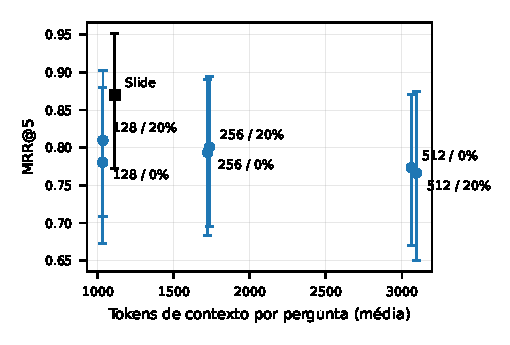
\includegraphics[width=\columnwidth]{compromisso.pdf}
\caption{MRR@5 contra o número médio de tokens de contexto por pergunta; barras indicam o IC de 95\,\% por \textit{bootstrap}. A linha de base por slide (quadrado) obtém a melhor ordenação com um dos menores custos.}
\label{fig:compromisso}
\end{figure}

Todas as configurações se abstiveram nas \NNaoRespondiveisTeste{} perguntas sem resposta (\AbstencaoCorretaSlide) e nenhuma citou trecho inexistente.
A fração de respostas com citação caiu para \ComCitacaoCGrdCom{} na janela de 512 tokens com sobreposição, contra \ComCitacaoSlide{} na segmentação por slide.
Por parte do curso, a maior diferença ocorreu em explicabilidade e equidade (Parte VII), onde o Recall@5 foi \RecallCincoSlideParteVII{} com slides e \RecallCincoCMedComParteVII{} com janelas de 256 tokens com sobreposição.

Os juízes concordaram com kappa ponderado de \KappaCorrecao{} em correção e \KappaFidelidade{} em fidelidade, e as médias de correção variaram de \CorrecaoCGrdSem{} a \CorrecaoSlide{} entre configurações.
Dos \NItensRespondiveisAmostra{} itens respondíveis da amostra, \NAcerto{} foram acertos, \NFalhaGeracao{} falhas de geração e \NFalhaRecuperacao{} falhas de recuperação, e nenhuma resposta foi inventada para pergunta sem resposta.

\section{Discussão e Limitações}
A vantagem da segmentação por slide na ordenação é coerente com o material: cada slide condensa um conceito, e as perguntas factuais têm, por construção do conjunto, a resposta em uma única página, de modo que o trecho estrutural casa semanticamente com a pergunta.
As janelas maiores ganham Recall@5 porque cada trecho cobre várias páginas e conta como relevante se qualquer uma delas for evidência, o que também explica a menor precisão e o custo maior.
Na Parte VII, uma explicação provável é que conteúdos distribuídos por slides consecutivos, como as tabelas comparativas de métricas, sejam mais bem cobertos por janelas que unem páginas vizinhas.
A queda na fração de citações com trechos de 512 tokens é compatível com a dificuldade de modelos pequenos em usar contextos longos~\cite{liu2024lost}.
Como as falhas de geração superaram as de recuperação na amostra, ampliar o contexto tende a ter retorno limitado, e a hipótese a testar é que um gerador maior tenha efeito maior que a troca de segmentação.

O estudo não demonstra superioridade de nenhuma configuração: com \NRespondiveisTeste{} perguntas respondíveis, os intervalos das diferenças incluem zero ou tocam nele, e os resultados devem ser lidos como tendências.
A evidência anotada por página favorece a segmentação por slide no MRR e as janelas longas no Recall, e as perguntas foram escritas pelos próprios autores a partir dos slides.
A qualidade da resposta foi julgada por modelos de linguagem e não por humanos; juízes automáticos tendem a concordar entre si mais do que avaliadores humanos e podem compartilhar vieses~\cite{panickssery2024llm}, de modo que o kappa alto não garante validade, e a amostra de \NPerguntasAmostra{} perguntas não tem poder para comparar configurações.
Por fim, o estudo usa um único corpus, um único gerador de 3 bilhões de parâmetros e uma execução determinística, e a regra de seleção de $k$ fixou o maior valor candidato.

\section{Conclusão}
Em slides de aula em português, a segmentação estrutural por slide recuperou a evidência nas primeiras posições tão bem quanto janelas de tamanho fixo e com um dos menores custos de contexto.
Janelas longas aumentaram a cobertura das evidências, mas encareceram a geração e reduziram o uso de citações.
O gargalo observado esteve mais no gerador do que na recuperação.
Trabalhos futuros devem repetir o protocolo com mais perguntas, avaliação humana e geradores maiores.

\bibliographystyle{IEEEtran}
\bibliography{refs}

\end{document}
